% ---------------------------------------------------------------------------
% sec_theory_neurips_with_visuals.tex — condensed, formula-first version for the NeurIPS
% Interp4Discovery workshop template (5-page main text; this section ~3.5 pp).
% Drop-in: % ---------------------------------------------------------------------------
% sec_theory_neurips_with_visuals.tex — condensed, formula-first version for the NeurIPS
% Interp4Discovery workshop template (5-page main text; this section ~3.5 pp).
% Drop-in: % ---------------------------------------------------------------------------
% sec_theory_neurips_with_visuals.tex — condensed, formula-first version for the NeurIPS
% Interp4Discovery workshop template (5-page main text; this section ~3.5 pp).
% Drop-in: % ---------------------------------------------------------------------------
% sec_theory_neurips_with_visuals.tex — condensed, formula-first version for the NeurIPS
% Interp4Discovery workshop template (5-page main text; this section ~3.5 pp).
% Drop-in: \input{sec_theory_neurips_with_visuals} after the Introduction.
% Preamble needs: \newtheorem{proposition}{Proposition}  (guarded below)
% and the macros \E \Prob \ind from the v0.4 preamble.
% No experimental numerals. All \ref targets exist in main.tex v0.4.
% ---------------------------------------------------------------------------
\ifcsname proposition\endcsname\else\newtheorem{proposition}{Proposition}\fi
\providecommand{\E}{\mathbb{E}}
\providecommand{\Prob}{\mathbb{P}}
\providecommand{\ind}{\mathbf{1}}

\section{From explanation to controllable policy}
\label{sec:theory}

Whether a policy can be \emph{described} in readable language, whether the readable
variables are part of the mechanism that produces its actions, and whether writing to them
changes behavior predictably are three different properties:
\begin{equation}
\text{description} \;\neq\; \text{causal faithfulness} \;\neq\; \text{controllable intervention}.
\label{eq:hierarchy}
\end{equation}
This section states the criteria that separate them, as seven propositions the later sections
test \citep{rudin2019,doshivelez2017}.

\subsection{Objects and the four requirements}
\label{sec:theory:four}

Let $x_t$ be the observable state, $h_t$ the learned latent of a network policy
(Eq.~\ref{eq:intervene}), $b_t$ a named belief (Eq.~\ref{eq:belief}), $g_t$ the goal or
constraint state, $a_t$ the action, $\pi$ the \emph{executed} policy, and $\hat\pi$ any
surrogate fitted afterwards to imitate or explain $\pi$. Interpretability is the profile
\begin{equation}
\mathcal{I}(\pi) \;=\; \big(F,\ S,\ S\!t,\ C\big),
\label{eq:profile}
\end{equation}
with faithfulness $F$ (Eq.~\ref{eq:faith}; \citealp{jacovi2020}), simulatability $S$
(Eq.~\ref{eq:simul}; \citealp{lipton2018}), stability $S\!t$ (Eq.~\ref{eq:stab}), and
\emph{controllability} $C$: a targeted change to the representation changes the policy
predictably and without unrequested side effects. None implies another,
\begin{equation}
S \not\Rightarrow F, \qquad F \not\Rightarrow S, \qquad
S\!t \not\Rightarrow \text{correct}, \qquad
\big(\Delta a \neq 0\big) \not\Rightarrow C,
\label{eq:nonimply}
\end{equation}
and quoting one for another is the slippage already documented for NLP faithfulness tests
\citep{parcalabescu2024} and RL saliency \citep{atrey2020}.

\begin{proposition}[Non-equivalence of interpretability criteria]
\label{prop:nonequiv}
Predictive agreement, causal faithfulness, stability, and controllability are distinct
properties. No one property is sufficient to establish the others without additional
structural assumptions.
\end{proposition}

\subsection{Three levels of causal integration}
\label{sec:theory:generations}

The three systems in this paper differ in where the interpretable object sits relative to
the executed path (Figure~\ref{fig:generations}).
\begin{align}
\textit{transparent layers:}\quad & h_t = f_\theta(x_{\le t}), \qquad a_t = \pi_\theta(h_t, g_t),
\label{eq:gen1}\\
\textit{post-hoc:}\quad & b_t = q_\phi(h_t), \qquad \hat a_t = \hat\pi(b_t),
\label{eq:gen2}\\
\textit{born legible:}\quad & b_t = B(x_{\le t}), \qquad a_t = \pi_{\text{leg}}(b_t, g_t).
\label{eq:gen3}
\end{align}
In Eq.~\ref{eq:gen1} legibility is supplied by structure around the network, a hierarchy of
decision rhythms \citep{sutton1999options,bacon2017option} and hard constraints
\citep{achiam2017}; the constraints govern $a_t$ without revealing the mechanism that proposed
it (\S\ref{sec:chrl}). In Eq.~\ref{eq:gen2} the explanation $q_\phi$ is fitted after the
policy, so agreement on visited states does not license the interventional claim,
\begin{equation}
\hat\pi(b_t) \approx \pi(h_t)
\quad\not\Rightarrow\quad
\pi\big(\operatorname{do}(b_t = b^{*})\big) = \pi^{*}(b^{*}),
\label{eq:noimply}
\end{equation}
because the semantics of $b_t$ were read off the mechanism, not built into it
\citep{olah2020,atrey2020} (\S\ref{sec:interp}). In Eq.~\ref{eq:gen3} the belief is a declared
constructor (a Bayes filter over named regimes, Eq.~\ref{eq:belief}; \citealp{kaelbling1998})
and the small policy (a tree, Eq.~\ref{eq:tree}; \citealp{frosst2017}) \emph{is} the policy,
with no residual network for behavior to hide in: a concept bottleneck \citep{koh2020} whose
bottleneck is also the write surface (\S\ref{sec:crystal}).

\begin{proposition}[Causal integration]
\label{prop:integration}
Placing a named representation inside the executed decision path removes the
surrogate-to-policy gap, but does not by itself guarantee that the representation is
sufficient, correctly named, or safely writable.
\end{proposition}

\begin{figure}[t]
  \centering
  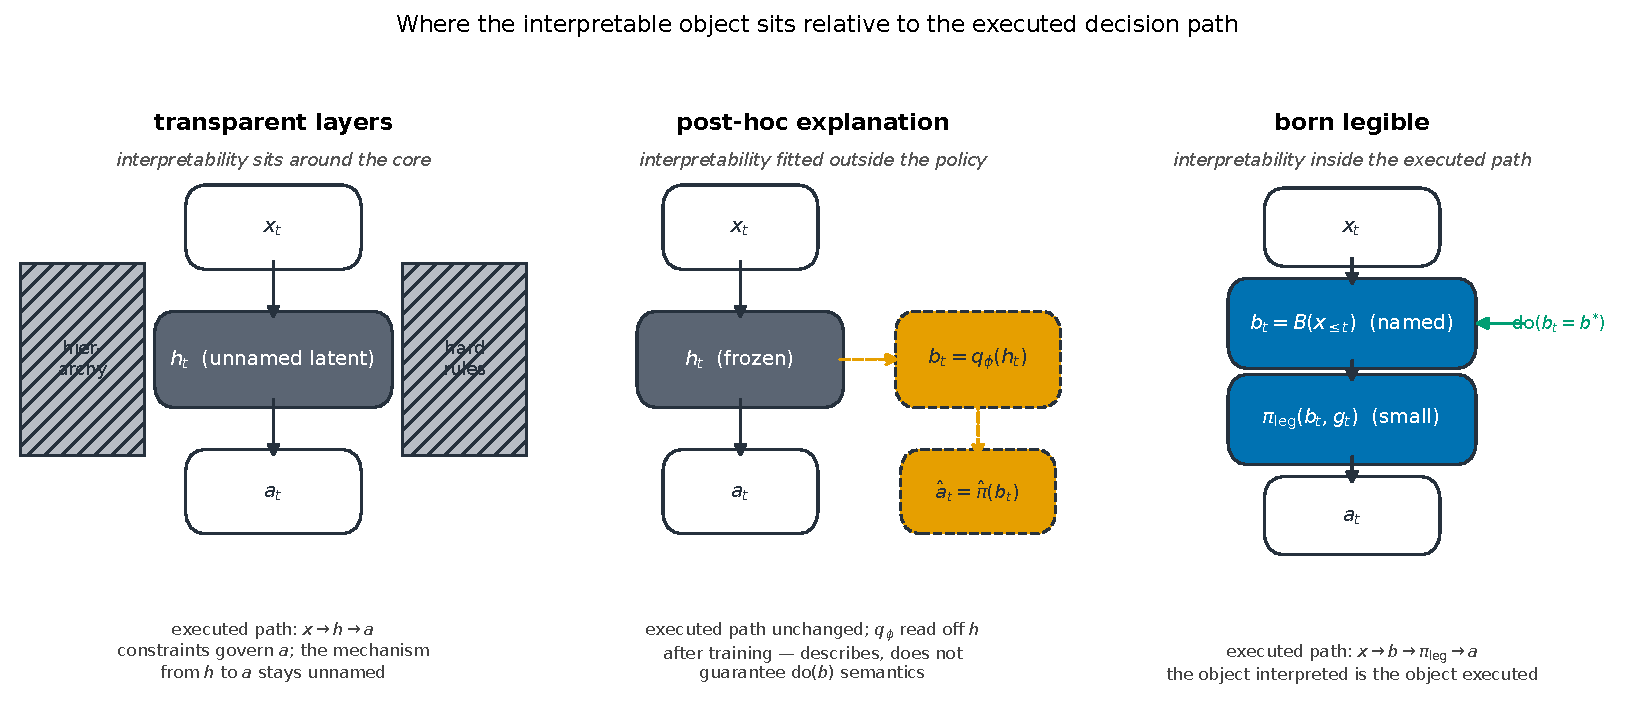
\includegraphics[width=.92\linewidth]{figures/fig_generations.pdf}
  \caption{Three levels of causal integration (Eqs.~\ref{eq:gen1}--\ref{eq:gen3}). Left:
  constraints sit around an unnamed latent $h$. Middle: an explanation $h\to b$ is fitted
  outside the executed path. Right: the named belief $b$ is inside the path, so the object
  interpreted is the object executed (Proposition~\ref{prop:integration}).}
  \label{fig:generations}
\end{figure}

\subsection{Observational versus interventional faithfulness}
\label{sec:theory:probe}

A probe is an instrument, and the first question is what it estimates. The observational
probe fits $\hat a_t = q(b_t)$ and reports recoverability under the visited distribution; the
interventional probe sets the belief by fiat \citep{pearl2009} and asks whether the action
follows the intended semantics:
\begin{equation}
F_{\text{obs}} = \Prob\big[\,q(b_t) = a_t\,\big],
\qquad
F_{\text{int}} = \Prob\big[\,\pi\big(\operatorname{do}(b_t = b^{*})\big) = a^{*}(b^{*})\,\big]
\;\;(\equiv \text{Eq.~\ref{eq:faith}}).
\label{eq:probes}
\end{equation}
The two estimands differ and may disagree in either direction. Even $F_{\text{int}}$ lies if
the intervention is too small. For a threshold policy, of which the certified rule
(Eq.~\ref{eq:rule}) is an instance,
\begin{equation}
a_t = \begin{cases} a^{-}, & b_t \le \tau\\ a^{+}, & b_t > \tau\end{cases}
\qquad\Longrightarrow\qquad
\pi(b_t + \delta) = \pi(b_t)\ \ \text{whenever } b_t + \delta \text{ does not cross } \tau,
\label{eq:threshold}
\end{equation}
so a fixed-size write reads $F_{\text{int}}=0$ on a policy that is entirely a function of
$b_t$. The failure is in the probe's support, and the repair is a matched contrast,
\begin{equation}
b^{-} < \tau < b^{+}, \qquad \text{compare } \pi(b^{-}) \text{ with } \pi(b^{+}),
\text{ all other state held fixed}.
\label{eq:contrast}
\end{equation}
Whether $b_t$ is coupled to $a_t$ at all is decided when the policy is fitted, not when it is
probed: under cold training the head may route around $b_t$; under a teacher warm start
\citep{ross2011dagger,rusu2016distillation} the coupling is installed first and the question
is whether optimization erodes it; under architectural construction there is nothing to
erode. Interpretability is partly a training property (\S\ref{sec:compare}).

\begin{proposition}[Probe dependence]
\label{prop:probe}
A faithfulness conclusion is valid only relative to the intervention support, the policy's
decision boundaries, and the training regime that couples the named representation to
action.
\end{proposition}

\subsection{Target effect, blast radius, refusal}
\label{sec:theory:control}

Influence is not control. For an intervention $I$ with intended target set $T$ and a
behavioral distance $D$,
\begin{equation}
\Delta_T(I) = D_T\big(\pi(\operatorname{do}(I)),\,\pi\big),
\qquad
B_{\neg T}(I) = D_{\neg T}\big(\pi(\operatorname{do}(I)),\,\pi\big),
\label{eq:target_blast}
\end{equation}
are the target effect and the blast radius. An intervention is actionable only if
\begin{equation}
\Delta_T(I) > \Delta_T(I_{\text{control}})
\qquad\text{and}\qquad
B_{\neg T}(I) \le \epsilon,
\label{eq:actionable}
\end{equation}
where $I_{\text{control}}$ is a matched intervention with no intended target (random
direction of equal magnitude, random coordinate, random primitive). The first condition is why
matched-random and joint controls are mandatory (\S\ref{sec:interpresults}); the second is what
a smeared latent cannot certify and a single-channel named memory can
(\S\ref{sec:crystal}, Eq.~\ref{eq:write}). When either cannot be certified the correct output
is a refusal:
\begin{equation}
\text{execute } I \iff
\operatorname{Support}(I)\ge\tau_s,\ \ B_{\neg T}(I)\le\tau_b,\ \ U(I)\le\tau_u;
\qquad \text{otherwise } \textsc{Refuse},
\label{eq:refuse}
\end{equation}
with $\operatorname{Support}$ the degree to which the intervened state lies in the training
distribution and $U$ the uncertainty of the estimated effect. The non-inferiority bar
(Eq.~\ref{eq:ni}) is one instance. A refusal is a result, not a missing one.

\begin{proposition}[Controlled intervention]
\label{prop:control}
An intervention is actionable only when its target effect exceeds an appropriate control and
its non-target effect remains within a declared blast-radius bound.
\end{proposition}

\begin{figure}[t]
  \centering
  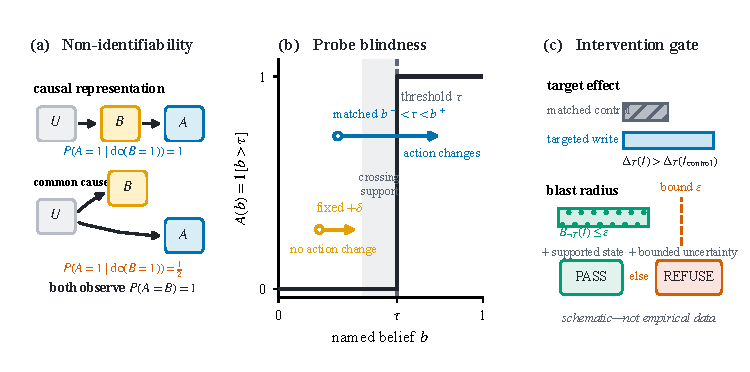
\includegraphics[width=.98\linewidth]{figures/fig_probe_control.pdf}
  \caption{Observational non-identifiability, threshold blindness, and controlled
  intervention. In panel (a), the binary common cause is
  $U\sim\operatorname{Bernoulli}(1/2)$ in both models. Observational agreement does not
  identify intervention response; a valid contrast crosses the decision boundary.
  Actionability additionally requires a target effect beyond its matched control, a non-target
  effect within the declared bound, supported state, and bounded uncertainty; otherwise
  \textsc{Refuse}.}
  \label{fig:probe-control}
\end{figure}

\subsection{When legibility binds}
\label{sec:theory:frontier}

For a description-length measure $L(\pi)$ (leaves, rules, or bits) and budget $K$,
\begin{equation}
\pi^{\star} = \arg\max_{\pi\in\Pi} \mathcal{R}(\pi),
\qquad
\pi^{\star}_K = \arg\max_{L(\pi)\le K} \mathcal{R}(\pi),
\qquad
D(K) = \mathcal{R}(\pi^{\star}) - \mathcal{R}(\pi^{\star}_K),
\label{eq:deficit}
\end{equation}
where $D(K)$ is the performance-side counterpart of the MDL deficit (Eq.~\ref{eq:mdl};
\citealp{rissanen1978}): that one is accuracy lost by a short story, this one is reward lost
by a short policy, and distillation results \citep{bastani2018viper} concern the first, not
the second. A measured $D(K)>0$ has three readings, only the last of which is a claim about
legibility:
\begin{equation}
\begin{aligned}
D(K)\approx 0 &\;\Rightarrow\; \text{the legible class is adequate};\\
D(K)>0,\ \text{falling with more search} &\;\Rightarrow\; \text{optimization was the binding constraint};\\
D(K)>0 \text{ after adequate search and capacity} &\;\Rightarrow\; \text{legibility itself binds}.
\end{aligned}
\label{eq:readings}
\end{equation}
The designed-market experiments (\S\ref{sec:polygon}) are built to separate these cases.
$L(\pi)$ counts leaves, rules, or bits, not the effort a person needs; the two can diverge.

\begin{proposition}[Conditional cost of legibility]
\label{prop:frontier}
The performance cost of legibility is not constant. It depends jointly on task complexity,
representation capacity, and optimization budget.
\end{proposition}

\begin{figure}[t]
  \centering
  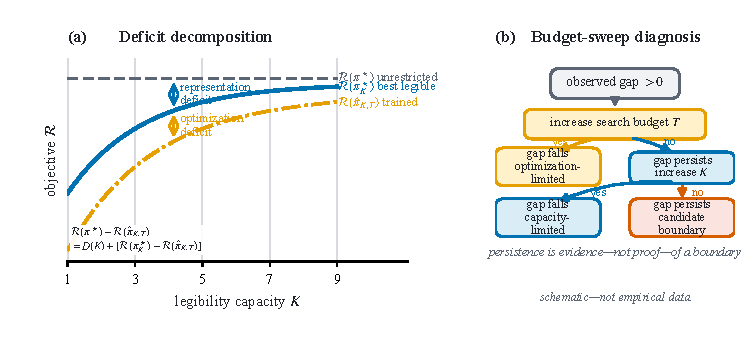
\includegraphics[width=.98\linewidth]{figures/fig_legibility_budget.pdf}
  \caption{Representation and optimization deficits under a legibility budget. The observed
  gap separates into $D(K)=\mathcal{R}(\pi^\star)-\mathcal{R}(\pi_K^\star)$ and the
  finite-optimization deficit
  $\mathcal{R}(\pi_K^\star)-\mathcal{R}(\hat\pi_{K,T})$. Sweeps over $T$ and then $K$
  diagnose which constraint binds but do not prove a boundary. Curves are schematic and
  contain no empirical values.}
  \label{fig:legibility-budget}
\end{figure}

\subsection{Legibility as governance, not alpha}
\label{sec:theory:finance}

Nothing here predicts that a legible policy earns more; the paper makes no alpha claim on
legibility's behalf. Its value enters the objective through risk, complexity, and
intervention uncertainty,
\begin{equation}
\max_{\pi}\ \E\big[R(\pi)\big] - \lambda_r\,\rho(\pi) - \lambda_c\,L(\pi) - \lambda_u\,U(\pi),
\label{eq:objective}
\end{equation}
with $\rho$ a risk functional such as drawdown (Eq.~\ref{eq:mdd}); the drawdown-penalized
reward (Eq.~\ref{eq:reward}) and hard constraints \citep{achiam2017} instantiate the first
penalty, the budget $K$ the second. Under Eq.~\ref{eq:objective} a legible policy can be
preferred at lower expected return because a risk budget can be verified rather than trusted,
an intervention has a declared blast radius, refusal is an available outcome, a modified
policy can be re-certified because the object certified is the object run, and every decision
is auditable to the variables that produced it \citep{rudin2019}. The certified rule
(\S\ref{sec:cert}) is scored on exactly this trade.

\begin{proposition}[Governance value]
\label{prop:governance}
In high-stakes sequential decisions, a legible policy may be preferable without producing
alpha when its measurable risk and governance benefits justify its performance cost.
\end{proposition}

\subsection{When scores are comparable}
\label{sec:theory:compare}

The measured axes form a vector, and \textsc{CrystalScore} (Eq.~\ref{eq:cs}) is its product:
\begin{equation}
\mathbf{C}(\pi) = \big[F(\pi),\ S(\pi),\ S\!t(\pi)\big],
\qquad
\textsc{CrystalScore}(\pi) = \prod_i \mathbf{C}_i(\pi).
\label{eq:vector}
\end{equation}
The product collapses on any failed axis, which is its virtue; it also equal-weights axes on
different scales, hides which axis failed, amplifies estimation error, and maps different
profiles to one number. The vector is the primary object; the scalar is admissible only when $\operatorname{Comparable}(\pi_i,\pi_j)=1$,
\begin{equation}
\begin{aligned}
\operatorname{Comparable}(\pi_i,\pi_j) \;=\; \ind\big[&\text{same substrate, split, period, units,}\\
&\text{policy object, estimators, and budget } K\big],
\end{aligned}
\label{eq:comparable}
\end{equation}
otherwise the two vectors are reported side by side and no scalar ratio is stated
\citep{hoffman2018,doshivelez2017} (\S\ref{sec:metrics}).

\begin{proposition}[Comparability]
\label{prop:comparable}
Composite interpretability scores support quantitative system comparison only when their
component estimands and evaluation substrates are compatible.
\end{proposition}

\paragraph{Empirical questions.}
The propositions are criteria, not results. The sections that follow ask, in construction
order: whether transparent layers expose the decisive computation (\S\ref{sec:chrl});
whether a post-hoc vocabulary is stable and whether targeted edits beat matched controls
(\S\ref{sec:interp}); whether probe design and training regime change the faithfulness
verdict (\S\ref{sec:metrics}, \S\ref{sec:compare}); whether a born-legible policy matches a
less constrained one at fixed $K$ and where the budget binds (\S\ref{sec:crystal},
\S\ref{sec:polygon}); whether a readable real-data rule buys risk without alpha
(\S\ref{sec:cert}); and whether the aggregate comparison meets Eq.~\ref{eq:comparable}
(\S\ref{sec:metrics}).
 after the Introduction.
% Preamble needs: \newtheorem{proposition}{Proposition}  (guarded below)
% and the macros \E \Prob \ind from the v0.4 preamble.
% No experimental numerals. All \ref targets exist in main.tex v0.4.
% ---------------------------------------------------------------------------
\ifcsname proposition\endcsname\else\newtheorem{proposition}{Proposition}\fi
\providecommand{\E}{\mathbb{E}}
\providecommand{\Prob}{\mathbb{P}}
\providecommand{\ind}{\mathbf{1}}

\section{From explanation to controllable policy}
\label{sec:theory}

Whether a policy can be \emph{described} in readable language, whether the readable
variables are part of the mechanism that produces its actions, and whether writing to them
changes behavior predictably are three different properties:
\begin{equation}
\text{description} \;\neq\; \text{causal faithfulness} \;\neq\; \text{controllable intervention}.
\label{eq:hierarchy}
\end{equation}
This section states the criteria that separate them, as seven propositions the later sections
test \citep{rudin2019,doshivelez2017}.

\subsection{Objects and the four requirements}
\label{sec:theory:four}

Let $x_t$ be the observable state, $h_t$ the learned latent of a network policy
(Eq.~\ref{eq:intervene}), $b_t$ a named belief (Eq.~\ref{eq:belief}), $g_t$ the goal or
constraint state, $a_t$ the action, $\pi$ the \emph{executed} policy, and $\hat\pi$ any
surrogate fitted afterwards to imitate or explain $\pi$. Interpretability is the profile
\begin{equation}
\mathcal{I}(\pi) \;=\; \big(F,\ S,\ S\!t,\ C\big),
\label{eq:profile}
\end{equation}
with faithfulness $F$ (Eq.~\ref{eq:faith}; \citealp{jacovi2020}), simulatability $S$
(Eq.~\ref{eq:simul}; \citealp{lipton2018}), stability $S\!t$ (Eq.~\ref{eq:stab}), and
\emph{controllability} $C$: a targeted change to the representation changes the policy
predictably and without unrequested side effects. None implies another,
\begin{equation}
S \not\Rightarrow F, \qquad F \not\Rightarrow S, \qquad
S\!t \not\Rightarrow \text{correct}, \qquad
\big(\Delta a \neq 0\big) \not\Rightarrow C,
\label{eq:nonimply}
\end{equation}
and quoting one for another is the slippage already documented for NLP faithfulness tests
\citep{parcalabescu2024} and RL saliency \citep{atrey2020}.

\begin{proposition}[Non-equivalence of interpretability criteria]
\label{prop:nonequiv}
Predictive agreement, causal faithfulness, stability, and controllability are distinct
properties. No one property is sufficient to establish the others without additional
structural assumptions.
\end{proposition}

\subsection{Three levels of causal integration}
\label{sec:theory:generations}

The three systems in this paper differ in where the interpretable object sits relative to
the executed path (Figure~\ref{fig:generations}).
\begin{align}
\textit{transparent layers:}\quad & h_t = f_\theta(x_{\le t}), \qquad a_t = \pi_\theta(h_t, g_t),
\label{eq:gen1}\\
\textit{post-hoc:}\quad & b_t = q_\phi(h_t), \qquad \hat a_t = \hat\pi(b_t),
\label{eq:gen2}\\
\textit{born legible:}\quad & b_t = B(x_{\le t}), \qquad a_t = \pi_{\text{leg}}(b_t, g_t).
\label{eq:gen3}
\end{align}
In Eq.~\ref{eq:gen1} legibility is supplied by structure around the network, a hierarchy of
decision rhythms \citep{sutton1999options,bacon2017option} and hard constraints
\citep{achiam2017}; the constraints govern $a_t$ without revealing the mechanism that proposed
it (\S\ref{sec:chrl}). In Eq.~\ref{eq:gen2} the explanation $q_\phi$ is fitted after the
policy, so agreement on visited states does not license the interventional claim,
\begin{equation}
\hat\pi(b_t) \approx \pi(h_t)
\quad\not\Rightarrow\quad
\pi\big(\operatorname{do}(b_t = b^{*})\big) = \pi^{*}(b^{*}),
\label{eq:noimply}
\end{equation}
because the semantics of $b_t$ were read off the mechanism, not built into it
\citep{olah2020,atrey2020} (\S\ref{sec:interp}). In Eq.~\ref{eq:gen3} the belief is a declared
constructor (a Bayes filter over named regimes, Eq.~\ref{eq:belief}; \citealp{kaelbling1998})
and the small policy (a tree, Eq.~\ref{eq:tree}; \citealp{frosst2017}) \emph{is} the policy,
with no residual network for behavior to hide in: a concept bottleneck \citep{koh2020} whose
bottleneck is also the write surface (\S\ref{sec:crystal}).

\begin{proposition}[Causal integration]
\label{prop:integration}
Placing a named representation inside the executed decision path removes the
surrogate-to-policy gap, but does not by itself guarantee that the representation is
sufficient, correctly named, or safely writable.
\end{proposition}

\begin{figure}[t]
  \centering
  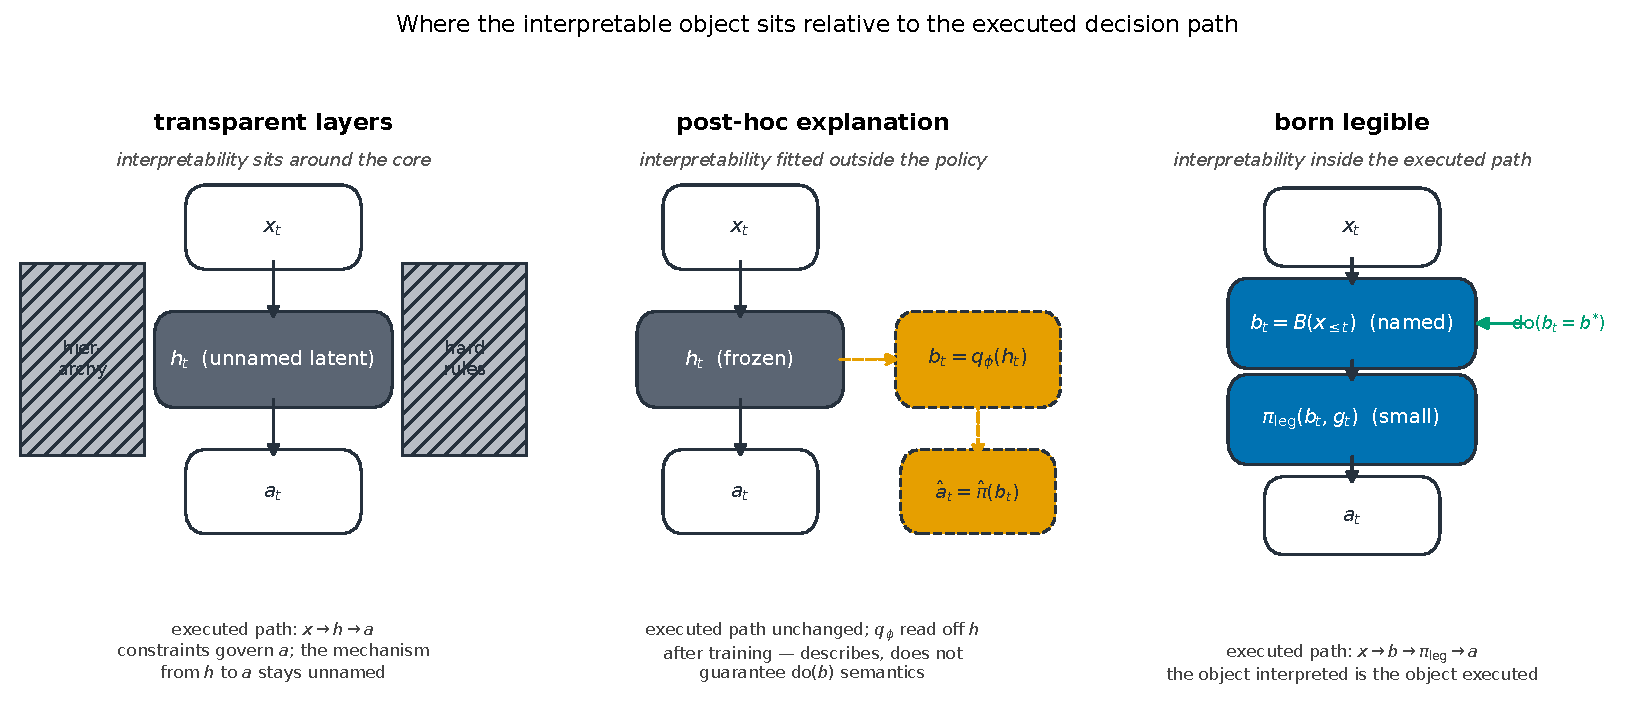
\includegraphics[width=.92\linewidth]{figures/fig_generations.pdf}
  \caption{Three levels of causal integration (Eqs.~\ref{eq:gen1}--\ref{eq:gen3}). Left:
  constraints sit around an unnamed latent $h$. Middle: an explanation $h\to b$ is fitted
  outside the executed path. Right: the named belief $b$ is inside the path, so the object
  interpreted is the object executed (Proposition~\ref{prop:integration}).}
  \label{fig:generations}
\end{figure}

\subsection{Observational versus interventional faithfulness}
\label{sec:theory:probe}

A probe is an instrument, and the first question is what it estimates. The observational
probe fits $\hat a_t = q(b_t)$ and reports recoverability under the visited distribution; the
interventional probe sets the belief by fiat \citep{pearl2009} and asks whether the action
follows the intended semantics:
\begin{equation}
F_{\text{obs}} = \Prob\big[\,q(b_t) = a_t\,\big],
\qquad
F_{\text{int}} = \Prob\big[\,\pi\big(\operatorname{do}(b_t = b^{*})\big) = a^{*}(b^{*})\,\big]
\;\;(\equiv \text{Eq.~\ref{eq:faith}}).
\label{eq:probes}
\end{equation}
The two estimands differ and may disagree in either direction. Even $F_{\text{int}}$ lies if
the intervention is too small. For a threshold policy, of which the certified rule
(Eq.~\ref{eq:rule}) is an instance,
\begin{equation}
a_t = \begin{cases} a^{-}, & b_t \le \tau\\ a^{+}, & b_t > \tau\end{cases}
\qquad\Longrightarrow\qquad
\pi(b_t + \delta) = \pi(b_t)\ \ \text{whenever } b_t + \delta \text{ does not cross } \tau,
\label{eq:threshold}
\end{equation}
so a fixed-size write reads $F_{\text{int}}=0$ on a policy that is entirely a function of
$b_t$. The failure is in the probe's support, and the repair is a matched contrast,
\begin{equation}
b^{-} < \tau < b^{+}, \qquad \text{compare } \pi(b^{-}) \text{ with } \pi(b^{+}),
\text{ all other state held fixed}.
\label{eq:contrast}
\end{equation}
Whether $b_t$ is coupled to $a_t$ at all is decided when the policy is fitted, not when it is
probed: under cold training the head may route around $b_t$; under a teacher warm start
\citep{ross2011dagger,rusu2016distillation} the coupling is installed first and the question
is whether optimization erodes it; under architectural construction there is nothing to
erode. Interpretability is partly a training property (\S\ref{sec:compare}).

\begin{proposition}[Probe dependence]
\label{prop:probe}
A faithfulness conclusion is valid only relative to the intervention support, the policy's
decision boundaries, and the training regime that couples the named representation to
action.
\end{proposition}

\subsection{Target effect, blast radius, refusal}
\label{sec:theory:control}

Influence is not control. For an intervention $I$ with intended target set $T$ and a
behavioral distance $D$,
\begin{equation}
\Delta_T(I) = D_T\big(\pi(\operatorname{do}(I)),\,\pi\big),
\qquad
B_{\neg T}(I) = D_{\neg T}\big(\pi(\operatorname{do}(I)),\,\pi\big),
\label{eq:target_blast}
\end{equation}
are the target effect and the blast radius. An intervention is actionable only if
\begin{equation}
\Delta_T(I) > \Delta_T(I_{\text{control}})
\qquad\text{and}\qquad
B_{\neg T}(I) \le \epsilon,
\label{eq:actionable}
\end{equation}
where $I_{\text{control}}$ is a matched intervention with no intended target (random
direction of equal magnitude, random coordinate, random primitive). The first condition is why
matched-random and joint controls are mandatory (\S\ref{sec:interpresults}); the second is what
a smeared latent cannot certify and a single-channel named memory can
(\S\ref{sec:crystal}, Eq.~\ref{eq:write}). When either cannot be certified the correct output
is a refusal:
\begin{equation}
\text{execute } I \iff
\operatorname{Support}(I)\ge\tau_s,\ \ B_{\neg T}(I)\le\tau_b,\ \ U(I)\le\tau_u;
\qquad \text{otherwise } \textsc{Refuse},
\label{eq:refuse}
\end{equation}
with $\operatorname{Support}$ the degree to which the intervened state lies in the training
distribution and $U$ the uncertainty of the estimated effect. The non-inferiority bar
(Eq.~\ref{eq:ni}) is one instance. A refusal is a result, not a missing one.

\begin{proposition}[Controlled intervention]
\label{prop:control}
An intervention is actionable only when its target effect exceeds an appropriate control and
its non-target effect remains within a declared blast-radius bound.
\end{proposition}

\begin{figure}[t]
  \centering
  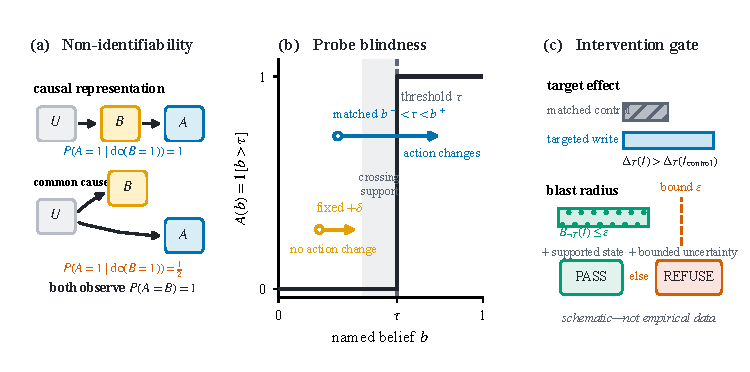
\includegraphics[width=.98\linewidth]{figures/fig_probe_control.pdf}
  \caption{Observational non-identifiability, threshold blindness, and controlled
  intervention. In panel (a), the binary common cause is
  $U\sim\operatorname{Bernoulli}(1/2)$ in both models. Observational agreement does not
  identify intervention response; a valid contrast crosses the decision boundary.
  Actionability additionally requires a target effect beyond its matched control, a non-target
  effect within the declared bound, supported state, and bounded uncertainty; otherwise
  \textsc{Refuse}.}
  \label{fig:probe-control}
\end{figure}

\subsection{When legibility binds}
\label{sec:theory:frontier}

For a description-length measure $L(\pi)$ (leaves, rules, or bits) and budget $K$,
\begin{equation}
\pi^{\star} = \arg\max_{\pi\in\Pi} \mathcal{R}(\pi),
\qquad
\pi^{\star}_K = \arg\max_{L(\pi)\le K} \mathcal{R}(\pi),
\qquad
D(K) = \mathcal{R}(\pi^{\star}) - \mathcal{R}(\pi^{\star}_K),
\label{eq:deficit}
\end{equation}
where $D(K)$ is the performance-side counterpart of the MDL deficit (Eq.~\ref{eq:mdl};
\citealp{rissanen1978}): that one is accuracy lost by a short story, this one is reward lost
by a short policy, and distillation results \citep{bastani2018viper} concern the first, not
the second. A measured $D(K)>0$ has three readings, only the last of which is a claim about
legibility:
\begin{equation}
\begin{aligned}
D(K)\approx 0 &\;\Rightarrow\; \text{the legible class is adequate};\\
D(K)>0,\ \text{falling with more search} &\;\Rightarrow\; \text{optimization was the binding constraint};\\
D(K)>0 \text{ after adequate search and capacity} &\;\Rightarrow\; \text{legibility itself binds}.
\end{aligned}
\label{eq:readings}
\end{equation}
The designed-market experiments (\S\ref{sec:polygon}) are built to separate these cases.
$L(\pi)$ counts leaves, rules, or bits, not the effort a person needs; the two can diverge.

\begin{proposition}[Conditional cost of legibility]
\label{prop:frontier}
The performance cost of legibility is not constant. It depends jointly on task complexity,
representation capacity, and optimization budget.
\end{proposition}

\begin{figure}[t]
  \centering
  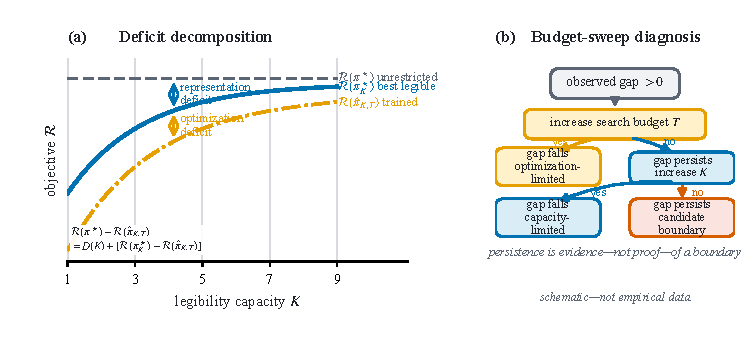
\includegraphics[width=.98\linewidth]{figures/fig_legibility_budget.pdf}
  \caption{Representation and optimization deficits under a legibility budget. The observed
  gap separates into $D(K)=\mathcal{R}(\pi^\star)-\mathcal{R}(\pi_K^\star)$ and the
  finite-optimization deficit
  $\mathcal{R}(\pi_K^\star)-\mathcal{R}(\hat\pi_{K,T})$. Sweeps over $T$ and then $K$
  diagnose which constraint binds but do not prove a boundary. Curves are schematic and
  contain no empirical values.}
  \label{fig:legibility-budget}
\end{figure}

\subsection{Legibility as governance, not alpha}
\label{sec:theory:finance}

Nothing here predicts that a legible policy earns more; the paper makes no alpha claim on
legibility's behalf. Its value enters the objective through risk, complexity, and
intervention uncertainty,
\begin{equation}
\max_{\pi}\ \E\big[R(\pi)\big] - \lambda_r\,\rho(\pi) - \lambda_c\,L(\pi) - \lambda_u\,U(\pi),
\label{eq:objective}
\end{equation}
with $\rho$ a risk functional such as drawdown (Eq.~\ref{eq:mdd}); the drawdown-penalized
reward (Eq.~\ref{eq:reward}) and hard constraints \citep{achiam2017} instantiate the first
penalty, the budget $K$ the second. Under Eq.~\ref{eq:objective} a legible policy can be
preferred at lower expected return because a risk budget can be verified rather than trusted,
an intervention has a declared blast radius, refusal is an available outcome, a modified
policy can be re-certified because the object certified is the object run, and every decision
is auditable to the variables that produced it \citep{rudin2019}. The certified rule
(\S\ref{sec:cert}) is scored on exactly this trade.

\begin{proposition}[Governance value]
\label{prop:governance}
In high-stakes sequential decisions, a legible policy may be preferable without producing
alpha when its measurable risk and governance benefits justify its performance cost.
\end{proposition}

\subsection{When scores are comparable}
\label{sec:theory:compare}

The measured axes form a vector, and \textsc{CrystalScore} (Eq.~\ref{eq:cs}) is its product:
\begin{equation}
\mathbf{C}(\pi) = \big[F(\pi),\ S(\pi),\ S\!t(\pi)\big],
\qquad
\textsc{CrystalScore}(\pi) = \prod_i \mathbf{C}_i(\pi).
\label{eq:vector}
\end{equation}
The product collapses on any failed axis, which is its virtue; it also equal-weights axes on
different scales, hides which axis failed, amplifies estimation error, and maps different
profiles to one number. The vector is the primary object; the scalar is admissible only when $\operatorname{Comparable}(\pi_i,\pi_j)=1$,
\begin{equation}
\begin{aligned}
\operatorname{Comparable}(\pi_i,\pi_j) \;=\; \ind\big[&\text{same substrate, split, period, units,}\\
&\text{policy object, estimators, and budget } K\big],
\end{aligned}
\label{eq:comparable}
\end{equation}
otherwise the two vectors are reported side by side and no scalar ratio is stated
\citep{hoffman2018,doshivelez2017} (\S\ref{sec:metrics}).

\begin{proposition}[Comparability]
\label{prop:comparable}
Composite interpretability scores support quantitative system comparison only when their
component estimands and evaluation substrates are compatible.
\end{proposition}

\paragraph{Empirical questions.}
The propositions are criteria, not results. The sections that follow ask, in construction
order: whether transparent layers expose the decisive computation (\S\ref{sec:chrl});
whether a post-hoc vocabulary is stable and whether targeted edits beat matched controls
(\S\ref{sec:interp}); whether probe design and training regime change the faithfulness
verdict (\S\ref{sec:metrics}, \S\ref{sec:compare}); whether a born-legible policy matches a
less constrained one at fixed $K$ and where the budget binds (\S\ref{sec:crystal},
\S\ref{sec:polygon}); whether a readable real-data rule buys risk without alpha
(\S\ref{sec:cert}); and whether the aggregate comparison meets Eq.~\ref{eq:comparable}
(\S\ref{sec:metrics}).
 after the Introduction.
% Preamble needs: \newtheorem{proposition}{Proposition}  (guarded below)
% and the macros \E \Prob \ind from the v0.4 preamble.
% No experimental numerals. All \ref targets exist in main.tex v0.4.
% ---------------------------------------------------------------------------
\ifcsname proposition\endcsname\else\newtheorem{proposition}{Proposition}\fi
\providecommand{\E}{\mathbb{E}}
\providecommand{\Prob}{\mathbb{P}}
\providecommand{\ind}{\mathbf{1}}

\section{From explanation to controllable policy}
\label{sec:theory}

Whether a policy can be \emph{described} in readable language, whether the readable
variables are part of the mechanism that produces its actions, and whether writing to them
changes behavior predictably are three different properties:
\begin{equation}
\text{description} \;\neq\; \text{causal faithfulness} \;\neq\; \text{controllable intervention}.
\label{eq:hierarchy}
\end{equation}
This section states the criteria that separate them, as seven propositions the later sections
test \citep{rudin2019,doshivelez2017}.

\subsection{Objects and the four requirements}
\label{sec:theory:four}

Let $x_t$ be the observable state, $h_t$ the learned latent of a network policy
(Eq.~\ref{eq:intervene}), $b_t$ a named belief (Eq.~\ref{eq:belief}), $g_t$ the goal or
constraint state, $a_t$ the action, $\pi$ the \emph{executed} policy, and $\hat\pi$ any
surrogate fitted afterwards to imitate or explain $\pi$. Interpretability is the profile
\begin{equation}
\mathcal{I}(\pi) \;=\; \big(F,\ S,\ S\!t,\ C\big),
\label{eq:profile}
\end{equation}
with faithfulness $F$ (Eq.~\ref{eq:faith}; \citealp{jacovi2020}), simulatability $S$
(Eq.~\ref{eq:simul}; \citealp{lipton2018}), stability $S\!t$ (Eq.~\ref{eq:stab}), and
\emph{controllability} $C$: a targeted change to the representation changes the policy
predictably and without unrequested side effects. None implies another,
\begin{equation}
S \not\Rightarrow F, \qquad F \not\Rightarrow S, \qquad
S\!t \not\Rightarrow \text{correct}, \qquad
\big(\Delta a \neq 0\big) \not\Rightarrow C,
\label{eq:nonimply}
\end{equation}
and quoting one for another is the slippage already documented for NLP faithfulness tests
\citep{parcalabescu2024} and RL saliency \citep{atrey2020}.

\begin{proposition}[Non-equivalence of interpretability criteria]
\label{prop:nonequiv}
Predictive agreement, causal faithfulness, stability, and controllability are distinct
properties. No one property is sufficient to establish the others without additional
structural assumptions.
\end{proposition}

\subsection{Three levels of causal integration}
\label{sec:theory:generations}

The three systems in this paper differ in where the interpretable object sits relative to
the executed path (Figure~\ref{fig:generations}).
\begin{align}
\textit{transparent layers:}\quad & h_t = f_\theta(x_{\le t}), \qquad a_t = \pi_\theta(h_t, g_t),
\label{eq:gen1}\\
\textit{post-hoc:}\quad & b_t = q_\phi(h_t), \qquad \hat a_t = \hat\pi(b_t),
\label{eq:gen2}\\
\textit{born legible:}\quad & b_t = B(x_{\le t}), \qquad a_t = \pi_{\text{leg}}(b_t, g_t).
\label{eq:gen3}
\end{align}
In Eq.~\ref{eq:gen1} legibility is supplied by structure around the network, a hierarchy of
decision rhythms \citep{sutton1999options,bacon2017option} and hard constraints
\citep{achiam2017}; the constraints govern $a_t$ without revealing the mechanism that proposed
it (\S\ref{sec:chrl}). In Eq.~\ref{eq:gen2} the explanation $q_\phi$ is fitted after the
policy, so agreement on visited states does not license the interventional claim,
\begin{equation}
\hat\pi(b_t) \approx \pi(h_t)
\quad\not\Rightarrow\quad
\pi\big(\operatorname{do}(b_t = b^{*})\big) = \pi^{*}(b^{*}),
\label{eq:noimply}
\end{equation}
because the semantics of $b_t$ were read off the mechanism, not built into it
\citep{olah2020,atrey2020} (\S\ref{sec:interp}). In Eq.~\ref{eq:gen3} the belief is a declared
constructor (a Bayes filter over named regimes, Eq.~\ref{eq:belief}; \citealp{kaelbling1998})
and the small policy (a tree, Eq.~\ref{eq:tree}; \citealp{frosst2017}) \emph{is} the policy,
with no residual network for behavior to hide in: a concept bottleneck \citep{koh2020} whose
bottleneck is also the write surface (\S\ref{sec:crystal}).

\begin{proposition}[Causal integration]
\label{prop:integration}
Placing a named representation inside the executed decision path removes the
surrogate-to-policy gap, but does not by itself guarantee that the representation is
sufficient, correctly named, or safely writable.
\end{proposition}

\begin{figure}[t]
  \centering
  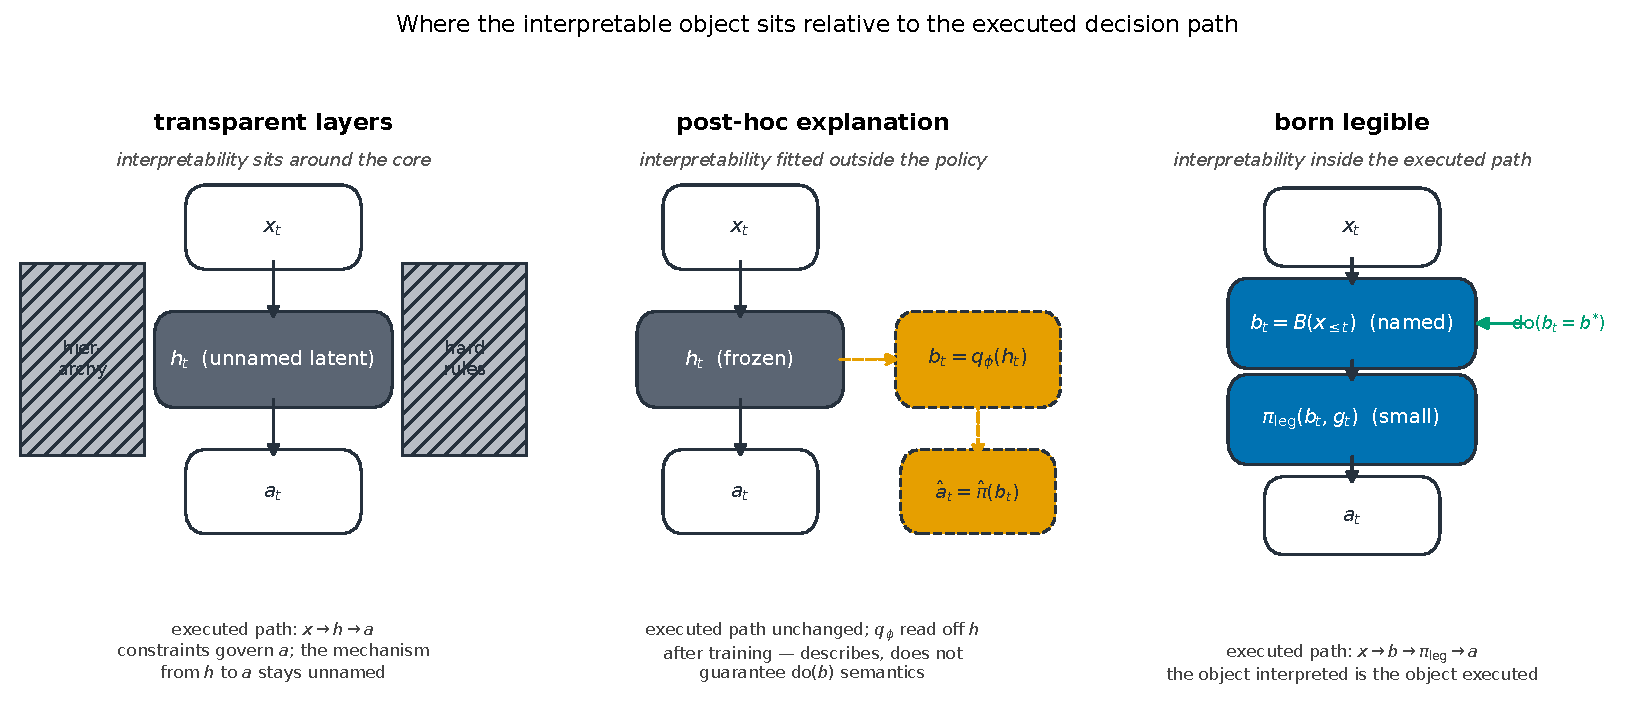
\includegraphics[width=.92\linewidth]{figures/fig_generations.pdf}
  \caption{Three levels of causal integration (Eqs.~\ref{eq:gen1}--\ref{eq:gen3}). Left:
  constraints sit around an unnamed latent $h$. Middle: an explanation $h\to b$ is fitted
  outside the executed path. Right: the named belief $b$ is inside the path, so the object
  interpreted is the object executed (Proposition~\ref{prop:integration}).}
  \label{fig:generations}
\end{figure}

\subsection{Observational versus interventional faithfulness}
\label{sec:theory:probe}

A probe is an instrument, and the first question is what it estimates. The observational
probe fits $\hat a_t = q(b_t)$ and reports recoverability under the visited distribution; the
interventional probe sets the belief by fiat \citep{pearl2009} and asks whether the action
follows the intended semantics:
\begin{equation}
F_{\text{obs}} = \Prob\big[\,q(b_t) = a_t\,\big],
\qquad
F_{\text{int}} = \Prob\big[\,\pi\big(\operatorname{do}(b_t = b^{*})\big) = a^{*}(b^{*})\,\big]
\;\;(\equiv \text{Eq.~\ref{eq:faith}}).
\label{eq:probes}
\end{equation}
The two estimands differ and may disagree in either direction. Even $F_{\text{int}}$ lies if
the intervention is too small. For a threshold policy, of which the certified rule
(Eq.~\ref{eq:rule}) is an instance,
\begin{equation}
a_t = \begin{cases} a^{-}, & b_t \le \tau\\ a^{+}, & b_t > \tau\end{cases}
\qquad\Longrightarrow\qquad
\pi(b_t + \delta) = \pi(b_t)\ \ \text{whenever } b_t + \delta \text{ does not cross } \tau,
\label{eq:threshold}
\end{equation}
so a fixed-size write reads $F_{\text{int}}=0$ on a policy that is entirely a function of
$b_t$. The failure is in the probe's support, and the repair is a matched contrast,
\begin{equation}
b^{-} < \tau < b^{+}, \qquad \text{compare } \pi(b^{-}) \text{ with } \pi(b^{+}),
\text{ all other state held fixed}.
\label{eq:contrast}
\end{equation}
Whether $b_t$ is coupled to $a_t$ at all is decided when the policy is fitted, not when it is
probed: under cold training the head may route around $b_t$; under a teacher warm start
\citep{ross2011dagger,rusu2016distillation} the coupling is installed first and the question
is whether optimization erodes it; under architectural construction there is nothing to
erode. Interpretability is partly a training property (\S\ref{sec:compare}).

\begin{proposition}[Probe dependence]
\label{prop:probe}
A faithfulness conclusion is valid only relative to the intervention support, the policy's
decision boundaries, and the training regime that couples the named representation to
action.
\end{proposition}

\subsection{Target effect, blast radius, refusal}
\label{sec:theory:control}

Influence is not control. For an intervention $I$ with intended target set $T$ and a
behavioral distance $D$,
\begin{equation}
\Delta_T(I) = D_T\big(\pi(\operatorname{do}(I)),\,\pi\big),
\qquad
B_{\neg T}(I) = D_{\neg T}\big(\pi(\operatorname{do}(I)),\,\pi\big),
\label{eq:target_blast}
\end{equation}
are the target effect and the blast radius. An intervention is actionable only if
\begin{equation}
\Delta_T(I) > \Delta_T(I_{\text{control}})
\qquad\text{and}\qquad
B_{\neg T}(I) \le \epsilon,
\label{eq:actionable}
\end{equation}
where $I_{\text{control}}$ is a matched intervention with no intended target (random
direction of equal magnitude, random coordinate, random primitive). The first condition is why
matched-random and joint controls are mandatory (\S\ref{sec:interpresults}); the second is what
a smeared latent cannot certify and a single-channel named memory can
(\S\ref{sec:crystal}, Eq.~\ref{eq:write}). When either cannot be certified the correct output
is a refusal:
\begin{equation}
\text{execute } I \iff
\operatorname{Support}(I)\ge\tau_s,\ \ B_{\neg T}(I)\le\tau_b,\ \ U(I)\le\tau_u;
\qquad \text{otherwise } \textsc{Refuse},
\label{eq:refuse}
\end{equation}
with $\operatorname{Support}$ the degree to which the intervened state lies in the training
distribution and $U$ the uncertainty of the estimated effect. The non-inferiority bar
(Eq.~\ref{eq:ni}) is one instance. A refusal is a result, not a missing one.

\begin{proposition}[Controlled intervention]
\label{prop:control}
An intervention is actionable only when its target effect exceeds an appropriate control and
its non-target effect remains within a declared blast-radius bound.
\end{proposition}

\begin{figure}[t]
  \centering
  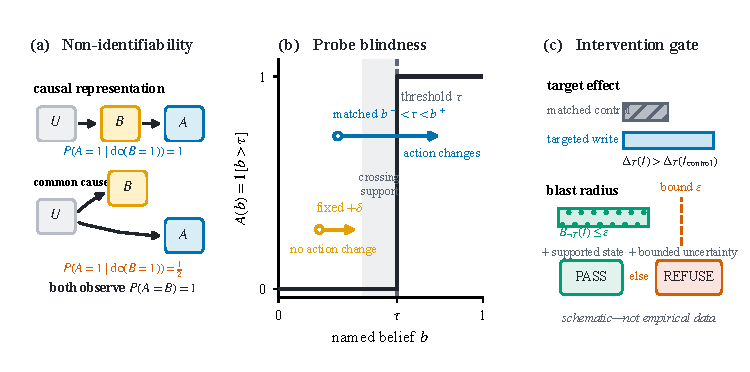
\includegraphics[width=.98\linewidth]{figures/fig_probe_control.pdf}
  \caption{Observational non-identifiability, threshold blindness, and controlled
  intervention. In panel (a), the binary common cause is
  $U\sim\operatorname{Bernoulli}(1/2)$ in both models. Observational agreement does not
  identify intervention response; a valid contrast crosses the decision boundary.
  Actionability additionally requires a target effect beyond its matched control, a non-target
  effect within the declared bound, supported state, and bounded uncertainty; otherwise
  \textsc{Refuse}.}
  \label{fig:probe-control}
\end{figure}

\subsection{When legibility binds}
\label{sec:theory:frontier}

For a description-length measure $L(\pi)$ (leaves, rules, or bits) and budget $K$,
\begin{equation}
\pi^{\star} = \arg\max_{\pi\in\Pi} \mathcal{R}(\pi),
\qquad
\pi^{\star}_K = \arg\max_{L(\pi)\le K} \mathcal{R}(\pi),
\qquad
D(K) = \mathcal{R}(\pi^{\star}) - \mathcal{R}(\pi^{\star}_K),
\label{eq:deficit}
\end{equation}
where $D(K)$ is the performance-side counterpart of the MDL deficit (Eq.~\ref{eq:mdl};
\citealp{rissanen1978}): that one is accuracy lost by a short story, this one is reward lost
by a short policy, and distillation results \citep{bastani2018viper} concern the first, not
the second. A measured $D(K)>0$ has three readings, only the last of which is a claim about
legibility:
\begin{equation}
\begin{aligned}
D(K)\approx 0 &\;\Rightarrow\; \text{the legible class is adequate};\\
D(K)>0,\ \text{falling with more search} &\;\Rightarrow\; \text{optimization was the binding constraint};\\
D(K)>0 \text{ after adequate search and capacity} &\;\Rightarrow\; \text{legibility itself binds}.
\end{aligned}
\label{eq:readings}
\end{equation}
The designed-market experiments (\S\ref{sec:polygon}) are built to separate these cases.
$L(\pi)$ counts leaves, rules, or bits, not the effort a person needs; the two can diverge.

\begin{proposition}[Conditional cost of legibility]
\label{prop:frontier}
The performance cost of legibility is not constant. It depends jointly on task complexity,
representation capacity, and optimization budget.
\end{proposition}

\begin{figure}[t]
  \centering
  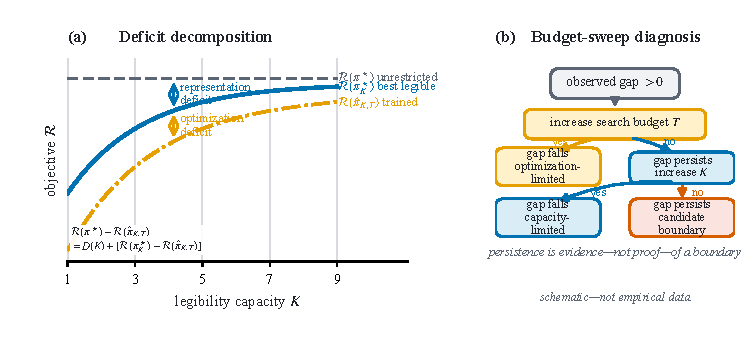
\includegraphics[width=.98\linewidth]{figures/fig_legibility_budget.pdf}
  \caption{Representation and optimization deficits under a legibility budget. The observed
  gap separates into $D(K)=\mathcal{R}(\pi^\star)-\mathcal{R}(\pi_K^\star)$ and the
  finite-optimization deficit
  $\mathcal{R}(\pi_K^\star)-\mathcal{R}(\hat\pi_{K,T})$. Sweeps over $T$ and then $K$
  diagnose which constraint binds but do not prove a boundary. Curves are schematic and
  contain no empirical values.}
  \label{fig:legibility-budget}
\end{figure}

\subsection{Legibility as governance, not alpha}
\label{sec:theory:finance}

Nothing here predicts that a legible policy earns more; the paper makes no alpha claim on
legibility's behalf. Its value enters the objective through risk, complexity, and
intervention uncertainty,
\begin{equation}
\max_{\pi}\ \E\big[R(\pi)\big] - \lambda_r\,\rho(\pi) - \lambda_c\,L(\pi) - \lambda_u\,U(\pi),
\label{eq:objective}
\end{equation}
with $\rho$ a risk functional such as drawdown (Eq.~\ref{eq:mdd}); the drawdown-penalized
reward (Eq.~\ref{eq:reward}) and hard constraints \citep{achiam2017} instantiate the first
penalty, the budget $K$ the second. Under Eq.~\ref{eq:objective} a legible policy can be
preferred at lower expected return because a risk budget can be verified rather than trusted,
an intervention has a declared blast radius, refusal is an available outcome, a modified
policy can be re-certified because the object certified is the object run, and every decision
is auditable to the variables that produced it \citep{rudin2019}. The certified rule
(\S\ref{sec:cert}) is scored on exactly this trade.

\begin{proposition}[Governance value]
\label{prop:governance}
In high-stakes sequential decisions, a legible policy may be preferable without producing
alpha when its measurable risk and governance benefits justify its performance cost.
\end{proposition}

\subsection{When scores are comparable}
\label{sec:theory:compare}

The measured axes form a vector, and \textsc{CrystalScore} (Eq.~\ref{eq:cs}) is its product:
\begin{equation}
\mathbf{C}(\pi) = \big[F(\pi),\ S(\pi),\ S\!t(\pi)\big],
\qquad
\textsc{CrystalScore}(\pi) = \prod_i \mathbf{C}_i(\pi).
\label{eq:vector}
\end{equation}
The product collapses on any failed axis, which is its virtue; it also equal-weights axes on
different scales, hides which axis failed, amplifies estimation error, and maps different
profiles to one number. The vector is the primary object; the scalar is admissible only when $\operatorname{Comparable}(\pi_i,\pi_j)=1$,
\begin{equation}
\begin{aligned}
\operatorname{Comparable}(\pi_i,\pi_j) \;=\; \ind\big[&\text{same substrate, split, period, units,}\\
&\text{policy object, estimators, and budget } K\big],
\end{aligned}
\label{eq:comparable}
\end{equation}
otherwise the two vectors are reported side by side and no scalar ratio is stated
\citep{hoffman2018,doshivelez2017} (\S\ref{sec:metrics}).

\begin{proposition}[Comparability]
\label{prop:comparable}
Composite interpretability scores support quantitative system comparison only when their
component estimands and evaluation substrates are compatible.
\end{proposition}

\paragraph{Empirical questions.}
The propositions are criteria, not results. The sections that follow ask, in construction
order: whether transparent layers expose the decisive computation (\S\ref{sec:chrl});
whether a post-hoc vocabulary is stable and whether targeted edits beat matched controls
(\S\ref{sec:interp}); whether probe design and training regime change the faithfulness
verdict (\S\ref{sec:metrics}, \S\ref{sec:compare}); whether a born-legible policy matches a
less constrained one at fixed $K$ and where the budget binds (\S\ref{sec:crystal},
\S\ref{sec:polygon}); whether a readable real-data rule buys risk without alpha
(\S\ref{sec:cert}); and whether the aggregate comparison meets Eq.~\ref{eq:comparable}
(\S\ref{sec:metrics}).
 after the Introduction.
% Preamble needs: \newtheorem{proposition}{Proposition}  (guarded below)
% and the macros \E \Prob \ind from the v0.4 preamble.
% No experimental numerals. All \ref targets exist in main.tex v0.4.
% ---------------------------------------------------------------------------
\ifcsname proposition\endcsname\else\newtheorem{proposition}{Proposition}\fi
\providecommand{\E}{\mathbb{E}}
\providecommand{\Prob}{\mathbb{P}}
\providecommand{\ind}{\mathbf{1}}

\section{From explanation to controllable policy}
\label{sec:theory}

Whether a policy can be \emph{described} in readable language, whether the readable
variables are part of the mechanism that produces its actions, and whether writing to them
changes behavior predictably are three different properties:
\begin{equation}
\text{description} \;\neq\; \text{causal faithfulness} \;\neq\; \text{controllable intervention}.
\label{eq:hierarchy}
\end{equation}
This section states the criteria that separate them, as seven propositions the later sections
test \citep{rudin2019,doshivelez2017}.

\subsection{Objects and the four requirements}
\label{sec:theory:four}

Let $x_t$ be the observable state, $h_t$ the learned latent of a network policy
(Eq.~\ref{eq:intervene}), $b_t$ a named belief (Eq.~\ref{eq:belief}), $g_t$ the goal or
constraint state, $a_t$ the action, $\pi$ the \emph{executed} policy, and $\hat\pi$ any
surrogate fitted afterwards to imitate or explain $\pi$. Interpretability is the profile
\begin{equation}
\mathcal{I}(\pi) \;=\; \big(F,\ S,\ S\!t,\ C\big),
\label{eq:profile}
\end{equation}
with faithfulness $F$ (Eq.~\ref{eq:faith}; \citealp{jacovi2020}), simulatability $S$
(Eq.~\ref{eq:simul}; \citealp{lipton2018}), stability $S\!t$ (Eq.~\ref{eq:stab}), and
\emph{controllability} $C$: a targeted change to the representation changes the policy
predictably and without unrequested side effects. None implies another,
\begin{equation}
S \not\Rightarrow F, \qquad F \not\Rightarrow S, \qquad
S\!t \not\Rightarrow \text{correct}, \qquad
\big(\Delta a \neq 0\big) \not\Rightarrow C,
\label{eq:nonimply}
\end{equation}
and quoting one for another is the slippage already documented for NLP faithfulness tests
\citep{parcalabescu2024} and RL saliency \citep{atrey2020}.

\begin{proposition}[Non-equivalence of interpretability criteria]
\label{prop:nonequiv}
Predictive agreement, causal faithfulness, stability, and controllability are distinct
properties. No one property is sufficient to establish the others without additional
structural assumptions.
\end{proposition}

\subsection{Three levels of causal integration}
\label{sec:theory:generations}

The three systems in this paper differ in where the interpretable object sits relative to
the executed path (Figure~\ref{fig:generations}).
\begin{align}
\textit{transparent layers:}\quad & h_t = f_\theta(x_{\le t}), \qquad a_t = \pi_\theta(h_t, g_t),
\label{eq:gen1}\\
\textit{post-hoc:}\quad & b_t = q_\phi(h_t), \qquad \hat a_t = \hat\pi(b_t),
\label{eq:gen2}\\
\textit{born legible:}\quad & b_t = B(x_{\le t}), \qquad a_t = \pi_{\text{leg}}(b_t, g_t).
\label{eq:gen3}
\end{align}
In Eq.~\ref{eq:gen1} legibility is supplied by structure around the network, a hierarchy of
decision rhythms \citep{sutton1999options,bacon2017option} and hard constraints
\citep{achiam2017}; the constraints govern $a_t$ without revealing the mechanism that proposed
it (\S\ref{sec:chrl}). In Eq.~\ref{eq:gen2} the explanation $q_\phi$ is fitted after the
policy, so agreement on visited states does not license the interventional claim,
\begin{equation}
\hat\pi(b_t) \approx \pi(h_t)
\quad\not\Rightarrow\quad
\pi\big(\operatorname{do}(b_t = b^{*})\big) = \pi^{*}(b^{*}),
\label{eq:noimply}
\end{equation}
because the semantics of $b_t$ were read off the mechanism, not built into it
\citep{olah2020,atrey2020} (\S\ref{sec:interp}). In Eq.~\ref{eq:gen3} the belief is a declared
constructor (a Bayes filter over named regimes, Eq.~\ref{eq:belief}; \citealp{kaelbling1998})
and the small policy (a tree, Eq.~\ref{eq:tree}; \citealp{frosst2017}) \emph{is} the policy,
with no residual network for behavior to hide in: a concept bottleneck \citep{koh2020} whose
bottleneck is also the write surface (\S\ref{sec:crystal}).

\begin{proposition}[Causal integration]
\label{prop:integration}
Placing a named representation inside the executed decision path removes the
surrogate-to-policy gap, but does not by itself guarantee that the representation is
sufficient, correctly named, or safely writable.
\end{proposition}

\begin{figure}[t]
  \centering
  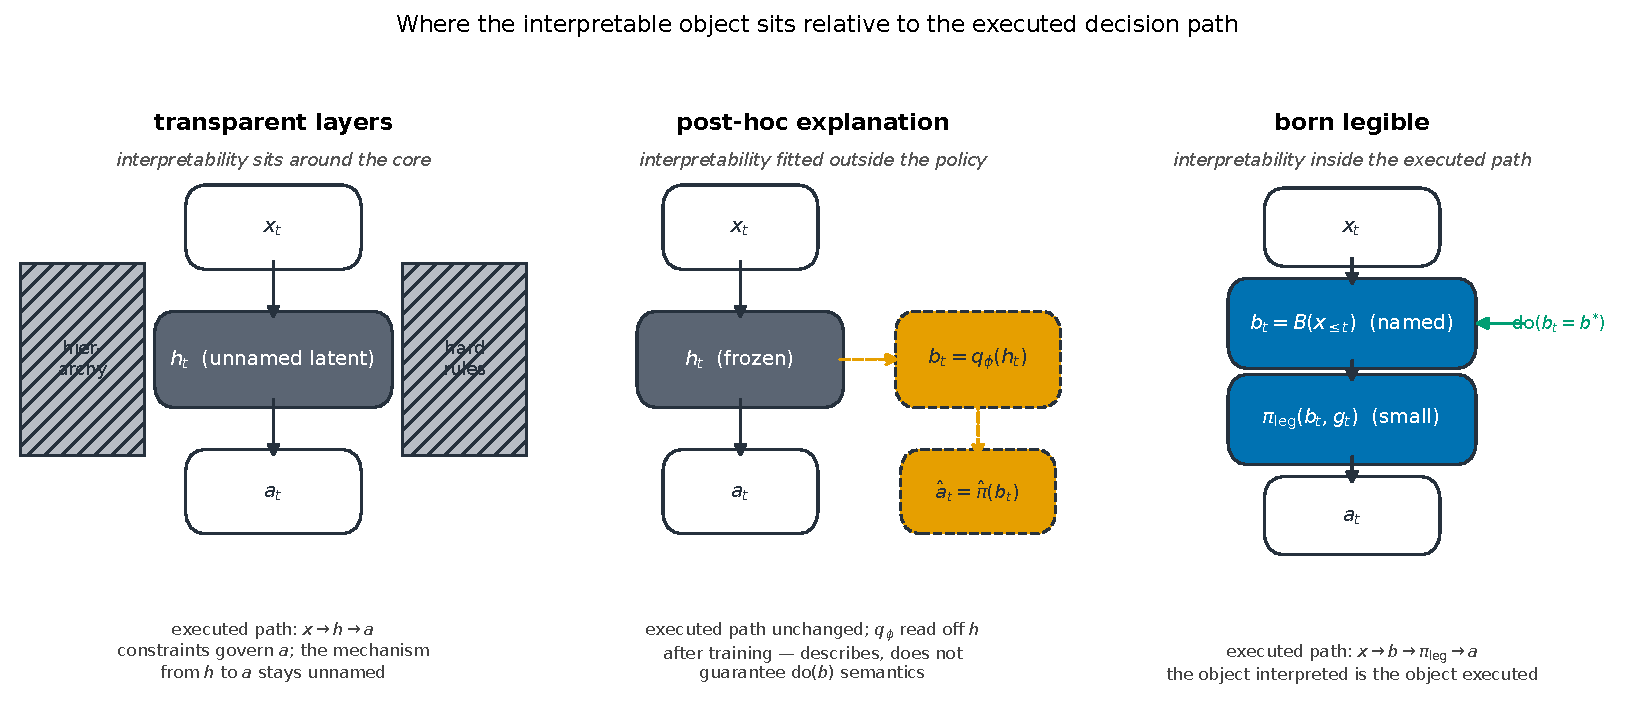
\includegraphics[width=.92\linewidth]{figures/fig_generations.pdf}
  \caption{Three levels of causal integration (Eqs.~\ref{eq:gen1}--\ref{eq:gen3}). Left:
  constraints sit around an unnamed latent $h$. Middle: an explanation $h\to b$ is fitted
  outside the executed path. Right: the named belief $b$ is inside the path, so the object
  interpreted is the object executed (Proposition~\ref{prop:integration}).}
  \label{fig:generations}
\end{figure}

\subsection{Observational versus interventional faithfulness}
\label{sec:theory:probe}

A probe is an instrument, and the first question is what it estimates. The observational
probe fits $\hat a_t = q(b_t)$ and reports recoverability under the visited distribution; the
interventional probe sets the belief by fiat \citep{pearl2009} and asks whether the action
follows the intended semantics:
\begin{equation}
F_{\text{obs}} = \Prob\big[\,q(b_t) = a_t\,\big],
\qquad
F_{\text{int}} = \Prob\big[\,\pi\big(\operatorname{do}(b_t = b^{*})\big) = a^{*}(b^{*})\,\big]
\;\;(\equiv \text{Eq.~\ref{eq:faith}}).
\label{eq:probes}
\end{equation}
The two estimands differ and may disagree in either direction. Even $F_{\text{int}}$ lies if
the intervention is too small. For a threshold policy, of which the certified rule
(Eq.~\ref{eq:rule}) is an instance,
\begin{equation}
a_t = \begin{cases} a^{-}, & b_t \le \tau\\ a^{+}, & b_t > \tau\end{cases}
\qquad\Longrightarrow\qquad
\pi(b_t + \delta) = \pi(b_t)\ \ \text{whenever } b_t + \delta \text{ does not cross } \tau,
\label{eq:threshold}
\end{equation}
so a fixed-size write reads $F_{\text{int}}=0$ on a policy that is entirely a function of
$b_t$. The failure is in the probe's support, and the repair is a matched contrast,
\begin{equation}
b^{-} < \tau < b^{+}, \qquad \text{compare } \pi(b^{-}) \text{ with } \pi(b^{+}),
\text{ all other state held fixed}.
\label{eq:contrast}
\end{equation}
Whether $b_t$ is coupled to $a_t$ at all is decided when the policy is fitted, not when it is
probed: under cold training the head may route around $b_t$; under a teacher warm start
\citep{ross2011dagger,rusu2016distillation} the coupling is installed first and the question
is whether optimization erodes it; under architectural construction there is nothing to
erode. Interpretability is partly a training property (\S\ref{sec:compare}).

\begin{proposition}[Probe dependence]
\label{prop:probe}
A faithfulness conclusion is valid only relative to the intervention support, the policy's
decision boundaries, and the training regime that couples the named representation to
action.
\end{proposition}

\subsection{Target effect, blast radius, refusal}
\label{sec:theory:control}

Influence is not control. For an intervention $I$ with intended target set $T$ and a
behavioral distance $D$,
\begin{equation}
\Delta_T(I) = D_T\big(\pi(\operatorname{do}(I)),\,\pi\big),
\qquad
B_{\neg T}(I) = D_{\neg T}\big(\pi(\operatorname{do}(I)),\,\pi\big),
\label{eq:target_blast}
\end{equation}
are the target effect and the blast radius. An intervention is actionable only if
\begin{equation}
\Delta_T(I) > \Delta_T(I_{\text{control}})
\qquad\text{and}\qquad
B_{\neg T}(I) \le \epsilon,
\label{eq:actionable}
\end{equation}
where $I_{\text{control}}$ is a matched intervention with no intended target (random
direction of equal magnitude, random coordinate, random primitive). The first condition is why
matched-random and joint controls are mandatory (\S\ref{sec:interpresults}); the second is what
a smeared latent cannot certify and a single-channel named memory can
(\S\ref{sec:crystal}, Eq.~\ref{eq:write}). When either cannot be certified the correct output
is a refusal:
\begin{equation}
\text{execute } I \iff
\operatorname{Support}(I)\ge\tau_s,\ \ B_{\neg T}(I)\le\tau_b,\ \ U(I)\le\tau_u;
\qquad \text{otherwise } \textsc{Refuse},
\label{eq:refuse}
\end{equation}
with $\operatorname{Support}$ the degree to which the intervened state lies in the training
distribution and $U$ the uncertainty of the estimated effect. The non-inferiority bar
(Eq.~\ref{eq:ni}) is one instance. A refusal is a result, not a missing one.

\begin{proposition}[Controlled intervention]
\label{prop:control}
An intervention is actionable only when its target effect exceeds an appropriate control and
its non-target effect remains within a declared blast-radius bound.
\end{proposition}

\begin{figure}[t]
  \centering
  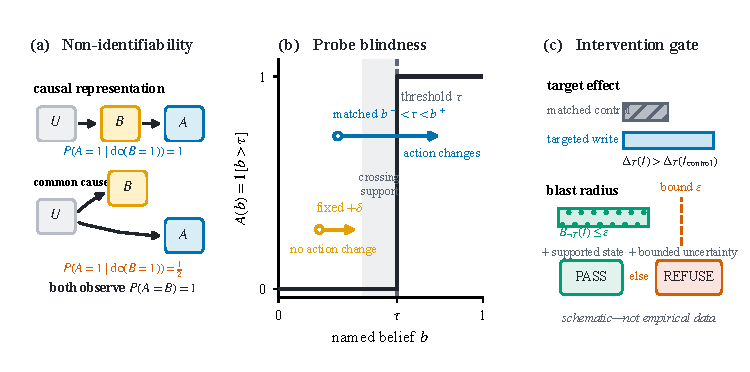
\includegraphics[width=.98\linewidth]{figures/fig_probe_control.pdf}
  \caption{Observational non-identifiability, threshold blindness, and controlled
  intervention. In panel (a), the binary common cause is
  $U\sim\operatorname{Bernoulli}(1/2)$ in both models. Observational agreement does not
  identify intervention response; a valid contrast crosses the decision boundary.
  Actionability additionally requires a target effect beyond its matched control, a non-target
  effect within the declared bound, supported state, and bounded uncertainty; otherwise
  \textsc{Refuse}.}
  \label{fig:probe-control}
\end{figure}

\subsection{When legibility binds}
\label{sec:theory:frontier}

For a description-length measure $L(\pi)$ (leaves, rules, or bits) and budget $K$,
\begin{equation}
\pi^{\star} = \arg\max_{\pi\in\Pi} \mathcal{R}(\pi),
\qquad
\pi^{\star}_K = \arg\max_{L(\pi)\le K} \mathcal{R}(\pi),
\qquad
D(K) = \mathcal{R}(\pi^{\star}) - \mathcal{R}(\pi^{\star}_K),
\label{eq:deficit}
\end{equation}
where $D(K)$ is the performance-side counterpart of the MDL deficit (Eq.~\ref{eq:mdl};
\citealp{rissanen1978}): that one is accuracy lost by a short story, this one is reward lost
by a short policy, and distillation results \citep{bastani2018viper} concern the first, not
the second. A measured $D(K)>0$ has three readings, only the last of which is a claim about
legibility:
\begin{equation}
\begin{aligned}
D(K)\approx 0 &\;\Rightarrow\; \text{the legible class is adequate};\\
D(K)>0,\ \text{falling with more search} &\;\Rightarrow\; \text{optimization was the binding constraint};\\
D(K)>0 \text{ after adequate search and capacity} &\;\Rightarrow\; \text{legibility itself binds}.
\end{aligned}
\label{eq:readings}
\end{equation}
The designed-market experiments (\S\ref{sec:polygon}) are built to separate these cases.
$L(\pi)$ counts leaves, rules, or bits, not the effort a person needs; the two can diverge.

\begin{proposition}[Conditional cost of legibility]
\label{prop:frontier}
The performance cost of legibility is not constant. It depends jointly on task complexity,
representation capacity, and optimization budget.
\end{proposition}

\begin{figure}[t]
  \centering
  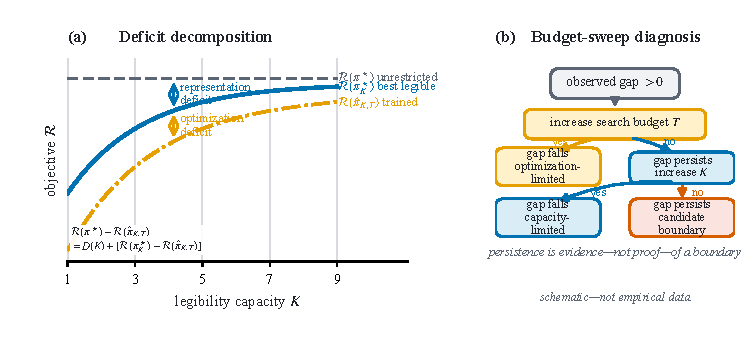
\includegraphics[width=.98\linewidth]{figures/fig_legibility_budget.pdf}
  \caption{Representation and optimization deficits under a legibility budget. The observed
  gap separates into $D(K)=\mathcal{R}(\pi^\star)-\mathcal{R}(\pi_K^\star)$ and the
  finite-optimization deficit
  $\mathcal{R}(\pi_K^\star)-\mathcal{R}(\hat\pi_{K,T})$. Sweeps over $T$ and then $K$
  diagnose which constraint binds but do not prove a boundary. Curves are schematic and
  contain no empirical values.}
  \label{fig:legibility-budget}
\end{figure}

\subsection{Legibility as governance, not alpha}
\label{sec:theory:finance}

Nothing here predicts that a legible policy earns more; the paper makes no alpha claim on
legibility's behalf. Its value enters the objective through risk, complexity, and
intervention uncertainty,
\begin{equation}
\max_{\pi}\ \E\big[R(\pi)\big] - \lambda_r\,\rho(\pi) - \lambda_c\,L(\pi) - \lambda_u\,U(\pi),
\label{eq:objective}
\end{equation}
with $\rho$ a risk functional such as drawdown (Eq.~\ref{eq:mdd}); the drawdown-penalized
reward (Eq.~\ref{eq:reward}) and hard constraints \citep{achiam2017} instantiate the first
penalty, the budget $K$ the second. Under Eq.~\ref{eq:objective} a legible policy can be
preferred at lower expected return because a risk budget can be verified rather than trusted,
an intervention has a declared blast radius, refusal is an available outcome, a modified
policy can be re-certified because the object certified is the object run, and every decision
is auditable to the variables that produced it \citep{rudin2019}. The certified rule
(\S\ref{sec:cert}) is scored on exactly this trade.

\begin{proposition}[Governance value]
\label{prop:governance}
In high-stakes sequential decisions, a legible policy may be preferable without producing
alpha when its measurable risk and governance benefits justify its performance cost.
\end{proposition}

\subsection{When scores are comparable}
\label{sec:theory:compare}

The measured axes form a vector, and \textsc{CrystalScore} (Eq.~\ref{eq:cs}) is its product:
\begin{equation}
\mathbf{C}(\pi) = \big[F(\pi),\ S(\pi),\ S\!t(\pi)\big],
\qquad
\textsc{CrystalScore}(\pi) = \prod_i \mathbf{C}_i(\pi).
\label{eq:vector}
\end{equation}
The product collapses on any failed axis, which is its virtue; it also equal-weights axes on
different scales, hides which axis failed, amplifies estimation error, and maps different
profiles to one number. The vector is the primary object; the scalar is admissible only when $\operatorname{Comparable}(\pi_i,\pi_j)=1$,
\begin{equation}
\begin{aligned}
\operatorname{Comparable}(\pi_i,\pi_j) \;=\; \ind\big[&\text{same substrate, split, period, units,}\\
&\text{policy object, estimators, and budget } K\big],
\end{aligned}
\label{eq:comparable}
\end{equation}
otherwise the two vectors are reported side by side and no scalar ratio is stated
\citep{hoffman2018,doshivelez2017} (\S\ref{sec:metrics}).

\begin{proposition}[Comparability]
\label{prop:comparable}
Composite interpretability scores support quantitative system comparison only when their
component estimands and evaluation substrates are compatible.
\end{proposition}

\paragraph{Empirical questions.}
The propositions are criteria, not results. The sections that follow ask, in construction
order: whether transparent layers expose the decisive computation (\S\ref{sec:chrl});
whether a post-hoc vocabulary is stable and whether targeted edits beat matched controls
(\S\ref{sec:interp}); whether probe design and training regime change the faithfulness
verdict (\S\ref{sec:metrics}, \S\ref{sec:compare}); whether a born-legible policy matches a
less constrained one at fixed $K$ and where the budget binds (\S\ref{sec:crystal},
\S\ref{sec:polygon}); whether a readable real-data rule buys risk without alpha
(\S\ref{sec:cert}); and whether the aggregate comparison meets Eq.~\ref{eq:comparable}
(\S\ref{sec:metrics}).
